\documentclass[pdf]{beamer}
\usepackage{graphicx}
\usepackage{pgfgantt}
\title{ESOP Garbage/Ancilla minimization}
\subtitle{}
\author{Micah Thornton \\ Josh Rendon}
\mode<presentation>{
    
    \usetheme{Warsaw}

}
\begin{document}



\begin{frame}
\titlepage
\end{frame}

\begin{frame}{Problem Statement}
    \begin{center}
    \textbf{Is it possible to classify a function as a Bijection by Quantum Synthesis alone?} \\ 
    -or-\\ 
    \textbf{Can we derive an algorithm to minimize the garbage and ancilla bits in a Quantum Cascade to determine whether or not a function can be synthesized without them?}
    \end{center}
\end{frame}

\begin{frame}{Background}
\begin{itemize}
   \item Bijections are functions which have a uniquely defined output for every possible input.
   \item Many circuits benefit from this characteristic. 
   \item Due to the definition of a bijection, any circuit which implements one is logically reversible. 
   \item This logical reversibility also allows the circuit to be represented as a quantum cascade (without any garbage or anscilla bits).
\end{itemize}
\end{frame}


\begin{frame}{Example}
\begin{columns}
\column{0.5\textwidth}
\vspace{-2 em}
\begin{center}
\textbf{Classical Half-Adder}
\end{center}
\vspace{-1 em}
\begin{figure}[ht]
\begin{center}
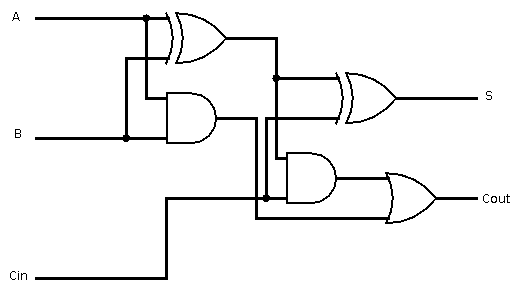
\includegraphics[scale=0.275]{figures/fulladder.png}
\end{center}
\end{figure}
\begin{block}{Classical Logic}
The logic Diagram represents a classical electronic ``Full-Adder'' circuit. Notice that inherently this circuit is not logically reversible. 
\end{block}
\column{0.5\textwidth}
\vspace{-2 em}
\begin{center}
\textbf{Quantum Half-Adder}
\end{center}
\vspace{-1 em}
\begin{figure}[ht]
\begin{center}
  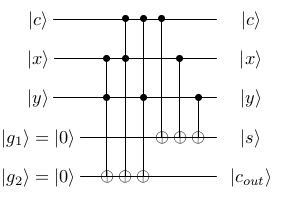
\includegraphics[scale=0.4]{figures/Full_adder_qc.png}
\end{center}
\end{figure}
\begin{block}{Quantum Logic}
If translated to quantum logic then two garbage input bits must be added in order to create a circuit that is truly logically reversible. 
\end{block}
\end{columns}

\end{frame}

\begin{frame}{Example 2}
\begin{columns}
\column{0.5\textwidth}
\vspace{-1 em}
\begin{center}
\textbf{Classical Circular Hash}
\end{center}
\vspace{-1 em}
\begin{figure}[ht]
\begin{center}
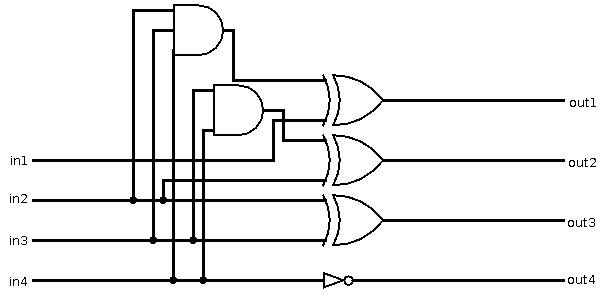
\includegraphics[scale=0.275]{figures/fbch.png}
\end{center}
\end{figure}
\begin{block}{Classical Logic}
In this case the logic is already reversible, note that this is usually the case when the number of inputs matches the number of outputs.
\end{block}
\column{0.5\textwidth}
\vspace{-1 em}
\begin{center}
\textbf{Quantum Circular Hash}
\end{center}
\begin{figure}[ht]
\begin{center}
\vspace{2 em}
  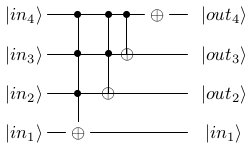
\includegraphics[scale=0.4]{figures/4-bit_circular_hash_qc.png}
\end{center}
\end{figure}
\begin{block}{Quantum Logic}
If translated to quantum logic no garbage input bits must be added, and the circuit is already reversible. 
\end{block}
\end{columns}

\end{frame}

\begin{frame}{Project Description}
\begin{enumerate}
    \item The development of an Ancilla/Garbage Minimization algorithm.
    \item The integration of our algorithm with a previous quantum synthesis algorithm ESOP.
    \item The creation of a categorizer which will accept a QUASM netlisting, generated by the previous steps, and decide whether it describes a classical bijection or not. 
    \item The generation of several circuits, in order to test our software system. 
\end{enumerate}
\end{frame}

\begin{frame}{Gantt Chart}

\begin{figure}[ht]
\begin{center}
\hspace{-4em}
  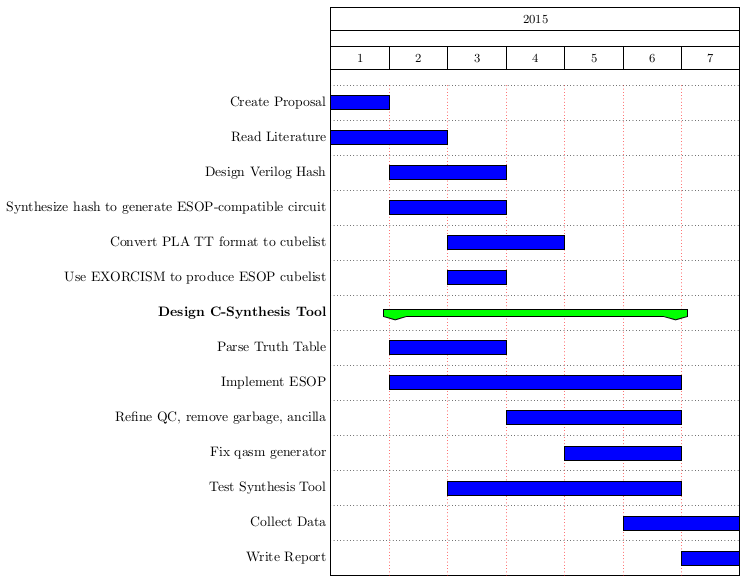
\includegraphics[scale=0.35]{figures/our_gantt.png}
\end{center}
\end{figure}

\end{frame}


\end{document}